\documentclass[10pt,a4paper]{article}
\usepackage[T1]{fontenc}
\usepackage[utf8]{inputenc}
\usepackage{newpxtext,newpxmath}
\usepackage{tgheros}
\setsansfont{texgyreheros-regular.otf}[BoldFont=texgyreheros-bold.otf,ItalicFont=texgyreheros-italic.otf,BoldItalicFont=texgyreheros-bolditalic.otf]
\usepackage{microtype}
\usepackage[a4paper,left=18mm,right=18mm,top=18mm,bottom=18mm,headheight=13pt,headsep=6mm,footskip=9mm]{geometry}
\usepackage{graphicx,xcolor,booktabs,tabularx,array,amsmath,enumitem}
\usepackage{tikz}
\usetikzlibrary{arrows.meta,calc}
\usepackage{fancyhdr,titlesec,caption,multicol}
\usepackage[pdfencoding=auto,psdextra]{hyperref}
\definecolor{ink}{HTML}{183B50}
\definecolor{teal}{HTML}{237F85}
\definecolor{gold}{HTML}{AA7939}
\definecolor{muted}{HTML}{5D6F79}
\definecolor{pale}{HTML}{EFF5F6}
\definecolor{rule}{HTML}{CEDADD}
\hypersetup{colorlinks=true,linkcolor=teal,urlcolor=teal,citecolor=teal,
 pdftitle={The Moving Observer: Does a moving viewpoint change the exoplanet sky?},
 pdfauthor={Biswajit Jana},pdfsubject={An illustrated research report from Finding Earth 2.0}}
\graphicspath{{images/}}
\setlength{\parindent}{0pt}\setlength{\parskip}{5.5pt}
\linespread{1.12}\setlength{\emergencystretch}{1.5em}\setlength{\columnsep}{7mm}
\setlist{nosep,leftmargin=1.2em,topsep=3pt}
\captionsetup{font={small,sf},labelfont={bf,color=ink},textfont={color=muted},skip=5pt,justification=raggedright,singlelinecheck=false}
\titleformat{\section}{\Large\bfseries\color{ink}}{}{0pt}{}
\titleformat{\subsection}{\large\bfseries\color{ink}}{}{0pt}{}
\titlespacing*{\section}{0pt}{0pt}{8pt}\titlespacing*{\subsection}{0pt}{10pt}{4pt}
\pagestyle{fancy}\fancyhf{}
\fancyhead[L]{\sffamily\scriptsize\color{muted}FINDING EARTH 2.0\quad /\quad THE MOVING OBSERVER}
\fancyhead[R]{\sffamily\scriptsize\color{muted}26 OCTOBER 2026\quad /\quad v7.4}
\fancyfoot[L]{\sffamily\scriptsize\color{muted}Biswajit Jana\quad\textbar\quad Independent research\quad\textbar\quad Not peer reviewed}
\fancyfoot[R]{\sffamily\scriptsize\color{muted}\thepage\ / 6}
\renewcommand{\headrulewidth}{.3pt}\renewcommand{\footrulewidth}{.3pt}
\renewcommand{\headrule}{\color{rule}\hrule width\headwidth height\headrulewidth}
\renewcommand{\footrule}{\color{rule}\hrule width\headwidth height\footrulewidth\vskip3pt}
\newcommand{\kicker}[1]{{\sffamily\small\bfseries\color{teal}#1}\par\vspace{4pt}}
\newcommand{\takeaway}[2]{\par\vspace{5pt}\begingroup\setlength{\fboxsep}{9pt}\colorbox{pale}{\parbox{\dimexpr\linewidth-18pt\relax}{\color{ink}\textbf{#1}\enspace #2}}\endgroup\par}
\newcommand{\figcap}[1]{\captionof{figure}{#1}}
\newcommand{\unit}[1]{\,\mathrm{#1}}
\newcommand{\source}[1]{{\sffamily\scriptsize\color{muted}#1}}
\newcommand{\reportpage}[2]{\newpage\kicker{#1}\section*{#2}}
\newcommand{\reference}[3]{\noindent\makebox[2.2em][l]{\textcolor{teal}{[#1]}}\parbox[t]{\dimexpr\linewidth-2.2em\relax}{\href{#3}{#2}}\par\vspace{3pt}}
\begin{document}\color{ink}
\begin{center}
 {\sffamily\small\bfseries\color{teal}AN ILLUSTRATED RESEARCH REPORT}\par\vspace{7pt}
 {\fontsize{25}{28}\selectfont\bfseries Does a moving viewpoint change\\the exoplanet sky?}\par\vspace{8pt}
 {\large A moving observer. Moving stars. Changing opportunities.}\par\vspace{9pt}
 {\large\textbf{Biswajit Jana}}\par
 {\sffamily\small Finding Earth 2.0\enspace\textbar\enspace Independent researcher and simulation author}
\end{center}
\vspace{5pt}
\textbf{The question.} As the Solar System moves through the Milky Way, could changing distances and sightlines make other planetary systems easier to detect? This report connects that curiosity to an interactive simulation and a limited, reproducible calculation. Both the observer and the target stars move; travelling farther does not by itself guarantee more discoveries.

\vspace{5pt}
\begin{minipage}[t]{.295\linewidth}\vspace{0pt}\setlength{\parskip}{3pt}
 \kicker{01 / THE ORIGINAL IDEA}
 \textbf{A: today. B: future.\\C: later future.}

 These positions illustrate a changing viewpoint along a Galactic orbit. They are epochs of the same observer, not three different stars.

 \vspace{5pt}{\fontsize{24}{26}\selectfont\color{teal}233}\enspace km/s\par
 \source{Adopted tangential speed.}

 \vspace{5pt}{\fontsize{24}{26}\selectfont\color{teal}0.0777}\enspace ly\par
 \source{Solar path in 100 years, at this speed: about 4,915 AU.}

 \vspace{5pt}{\fontsize{24}{26}\selectfont\color{teal}128,600}\par
 \source{Approximate model years needed to travel 100 light-years.}

 \vspace{8pt}\textbf{The crucial distinction}\par
 Solar travel relative to the Galaxy differs from motion relative to a nearby star. The latter changes our view of that star's planets.
\end{minipage}\hfill
\begin{minipage}[t]{.675\linewidth}\vspace{0pt}\setlength{\parskip}{3pt}
 \begin{tikzpicture}
  \node[inner sep=0,anchor=south west] (map) at (0,0) {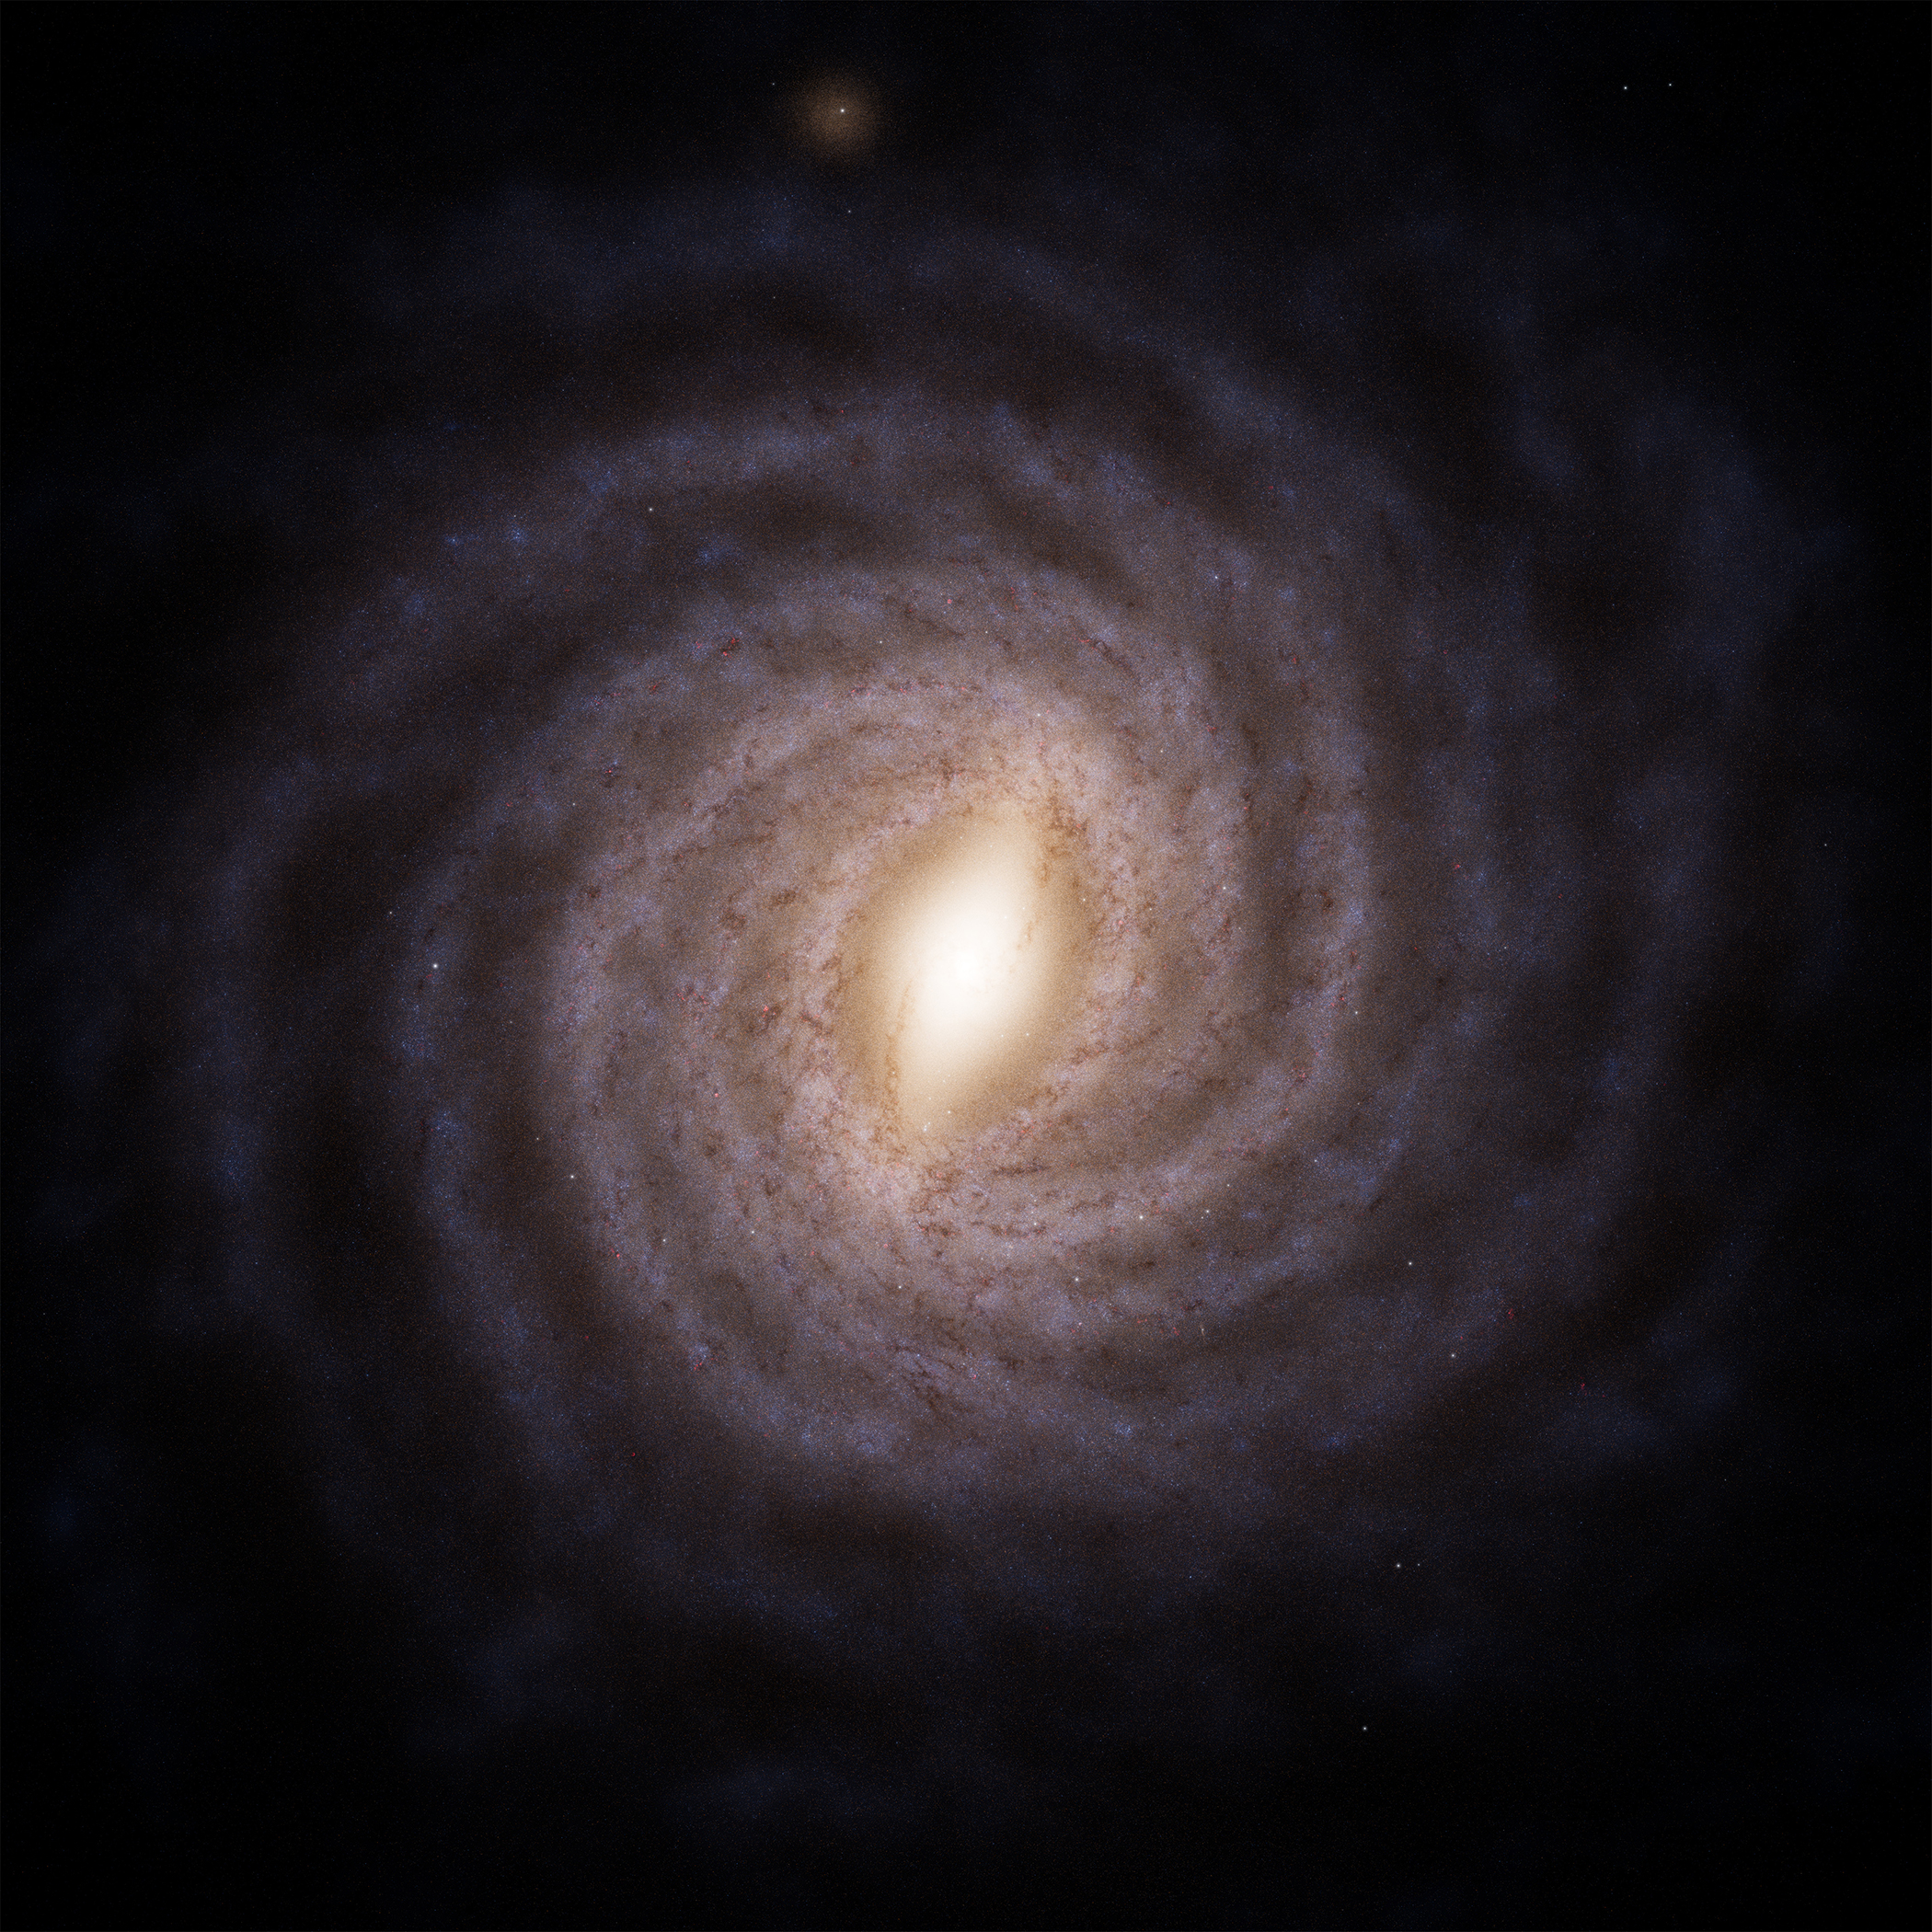
\includegraphics[width=\linewidth]{milky-way.jpg}};
  \begin{scope}[x={(map.south east)},y={(map.north west)}]
   \tikzset{tag/.style={font=\sffamily\fontsize{7}{8}\selectfont,text=white,fill=black,fill opacity=.65,text opacity=1,inner sep=3pt,align=left}}
   \draw[white,opacity=.65,line width=.4pt] (.49,.5)--(.58,.56);
   \node[tag,anchor=west] at (.57,.58) {Galactic centre};
   \draw[gold!65!white,dashed,line width=.7pt] (.5,.5) circle[radius=.205];
   \node[tag] at (.26,.47) {Sun's orbit\\$R_0\approx8.2$ kpc};
   \draw[-{Stealth[length=2mm]},gold!65!white,line width=1pt] (.5,.295) arc[start angle=270,end angle=236,radius=.205];
   \draw[-{Stealth[length=2mm]},gold!65!white,line width=1pt] (.386,.330) arc[start angle=236,end angle=204,radius=.205];
   \fill[gold!65!white] (.5,.295) circle[radius=.008];
   \fill[orange!70!white] (.386,.330) circle[radius=.008];
   \fill[cyan!65!white] (.313,.417) circle[radius=.008];
   \node[tag,anchor=north] at (.53,.265) {A / today};
   \node[tag,anchor=north east] at (.40,.30) {B / future};
   \node[tag,anchor=east] at (.29,.385) {C / later};
   \node[tag] at (.71,.78) {Perseus arm};
   \node[tag] at (.72,.65) {Sagittarius--Carina};
   \node[tag] at (.30,.64) {Scutum--Centaurus};
   \node[tag,anchor=west] at (.62,.32) {Local arm};
   \node[tag,anchor=west] at (.04,.92) {FACE-ON RECONSTRUCTION\\Observer epochs are schematic};
   \node[tag,anchor=south west] at (.04,.045) {Spiral structure is not a rigid track.\\The surrounding stars move too.};
  \end{scope}
 \end{tikzpicture}
 \figcap{A new annotated rendering of the original question. ESA/Gaia/DPAC, Stefan Payne-Wardenaar reconstruction [1], adapted with vector labels. Epoch positions, orbit and arm-name placement are schematic, not fitted boundaries or a predicted future sky.}
\end{minipage}

\takeaway{Working answer}{Relative motion can help or hinder a particular observation. In the selected century experiment, the imaging-accessibility sum changes by only \textbf{+0.0307\%}; the specified instrument-improvement scenario changes it much more. Neither result forecasts life or a number of discoveries.}
\vspace{5pt}
\source{Project, full methods, original discussion note and reproducible code: \href{https://biswajit1999.github.io/moving-observer/}{biswajit1999.github.io/moving-observer/}. This is a discussion report inviting expert criticism, not a claim of a new physical law.}

\reportpage{02 / FROM A MAP TO A MEASURABLE QUESTION}{Finding Earth 2.0 and changing sightlines}
The related \href{https://biswajit1999.github.io/finding-earth-2/}{Finding Earth 2.0 observatory} explores known exoplanets. Its saved 28 August 2026 analysis contains \textbf{6,354 confirmed planets and 4,764 host systems}, plus five Solar-System controls. This frozen snapshot is separate from the 1,387-source motion experiment on the next page.
\begin{center}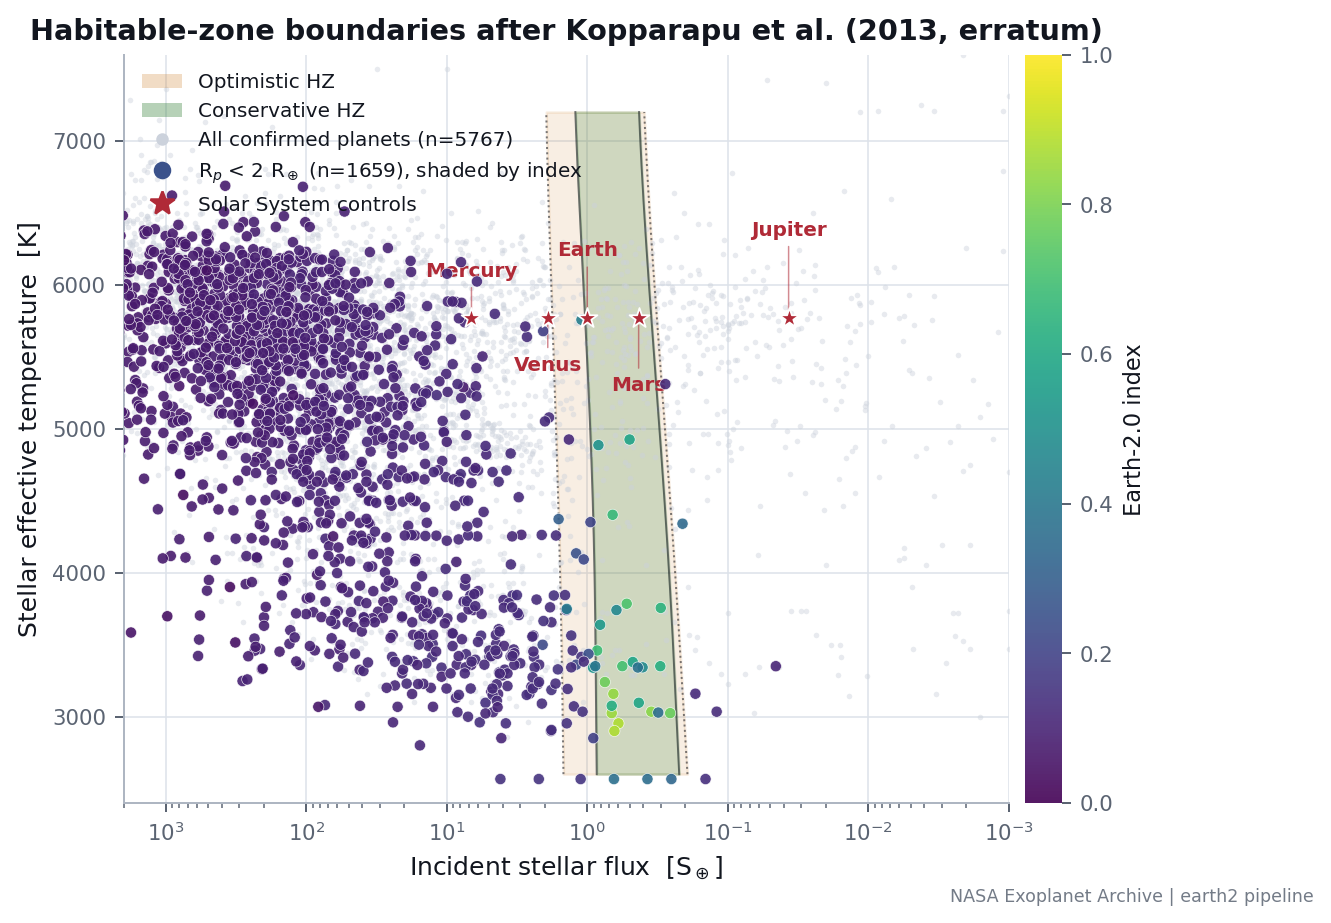
\includegraphics[width=.90\linewidth,height=84mm,keepaspectratio]{finding-earth-2.png}\end{center}
\figcap{The original saved Finding Earth 2.0 plot [2]: 5,767 planets with incident-flux and temperature data; 1,659 have radii below two Earth radii. The similarity index is not a probability of life. Habitable-zone placement alone does not establish surface habitability.}

\subsection*{Observer and target must share a reference frame}
Let $\mathbf r_i$ be a target's position and $\mathbf r_{\mathrm{obs}}$ the observer's position. Their relative position $\mathbf q_i$, distance $D_i$ and sightline $\widehat{\mathbf n}_i$ are
\begin{align}
 \mathbf r_{\mathrm{obs}}(t)&=\mathbf r_\odot(t)+\mathbf r_{\oplus/\odot}(t), &
 \mathbf q_i(t)&=\mathbf r_i(t)-\mathbf r_{\mathrm{obs}}(t),\label{eq:relative}\\
 D_i(t)&=\lVert\mathbf q_i(t)\rVert, &
 \widehat{\mathbf n}_i(t)&=\frac{\mathbf q_i(t)}{D_i(t)}.
\end{align}
For a sufficiently short interval,
\begin{equation}
 \Delta\theta_i\simeq\frac{\lVert\mathbf v_{i,\mathrm{rel},\perp}\rVert\,\Delta t}{D_i}.
\end{equation}
A transverse \emph{relative} speed of $30\unit{km\,s^{-1}}$ at $100\unit{ly}$ gives about $20.6$ arcseconds in 100 years. The Sun's total Galactic speed cannot be substituted for this relative transverse velocity.

\subsection*{A changed sightline is not automatically a new detection}
For a circular orbit, transit geometry depends on the orbital inclination $i$ to the sightline:
\begin{equation}
 b(t)=\frac{a\cos i(t)}{R_\star},\qquad
 |b|<1+\frac{R_p}{R_\star},\qquad
 P_{\mathrm{transit}}\simeq\frac{R_\star+R_p}{a}.
\end{equation}
Here $b$ is the impact parameter, $a$ the orbital radius, and $R_\star,R_p$ the stellar and planetary radii. An Earth--Sun analogue has an isotropic transit probability near $0.47\%$. Changing the view can open \emph{or close} a transit window; detection also requires adequate signal, cadence and orbital phase. Time-dependent Earth-transit-zone membership is already established research [3].

\reportpage{03 / THE REPRODUCIBLE EXPERIMENT}{How much does a century of motion change access?}
We ask a narrower question than ``how many planets will be found?'': for the \emph{same} nearby-source sample and hypothetical planet population, how does relative motion change single-visit direct-imaging accessibility? Four paired scenarios separate geometry from an assumed improvement in instrument thresholds.
\begin{center}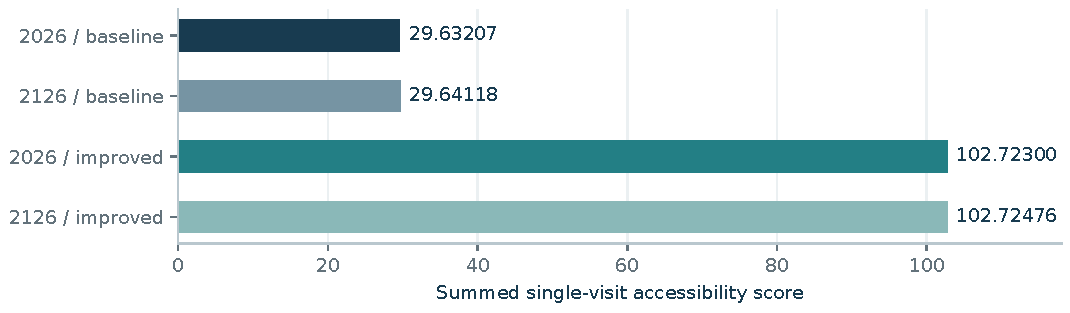
\includegraphics[width=\linewidth,height=55mm,keepaspectratio]{scores.pdf}\end{center}
\figcap{The baseline geometry change is visually tiny beside the chosen instrument change. Bar lengths are sums of conditional accessibility fractions, not planet counts. All four scenarios use the same \ReportSampleSize{} selected Gaia DR3 sources.}

\begin{minipage}[t]{.485\linewidth}\vspace{0pt}\setlength{\parskip}{3pt}
\subsection*{Data and assumptions}
Gaia DR3 selection [4]: parallax $\geq50$ mas, parallax signal-to-noise $>20$, measured radial velocity, RUWE $<1.4$ and at least ten visibility periods. This is not a complete nearby-star census.

Each source receives a hypothetical Earth-radius planet on a circular 1 AU orbit with geometric albedo 0.3. The score averages over isotropic orientations and phases.

\small\begin{tabularx}{\linewidth}{@{}Xrr@{}}\toprule
Threshold & Baseline & Improved\\\midrule
Inner working angle & 60 mas & 40 mas\\
Contrast floor & $10^{-10}$ & $5\!\times\!10^{-11}$\\
Planet magnitude limit & $G=30$ & $G=31$\\\bottomrule
\end{tabularx}\par\vspace{4pt}\normalsize
\end{minipage}\hfill
\begin{minipage}[t]{.485\linewidth}\vspace{0pt}\setlength{\parskip}{3pt}
\subsection*{Result and uncertainty}
The baseline sum changes from \textbf{\ReportBaselineInitial{} to \ReportBaselineFuture{}}. The motion contribution is
\[
 \Delta S_{\mathrm{motion}}=\ReportMotionScore\quad(\ReportMotionPercent\%).
\]
The assumed instrument change adds \textbf{\ReportInstrumentScore{}} at the initial epoch. These settings are sensitivity scenarios, not specifications for an approved telescope.

With \ReportDraws{} correlated astrometric draws per source, the formal 95\% interval for the motion difference is \textbf{\ReportMotionLow{} to \ReportMotionHigh{}}. It excludes population and instrument uncertainty, binary-system errors and cross-source systematics.
\end{minipage}

\subsection*{What the score actually measures}
For isotropic planet positions, $\cos\alpha$ is uniform. If the simultaneous angular-separation, contrast and magnitude conditions admit $[\alpha_{\min},\alpha_{\max}]$, then
\begin{equation}
 C_i=\frac{\cos\alpha_{\min}-\cos\alpha_{\max}}{2},\qquad
 S=\sum_{i=1}^{\ReportSampleSizeMath} C_i,
\end{equation}
with $C_i=0$ for an empty interval. Averaging over orientation removes sensitivity to the absolute sky direction. Thus this experiment tests distance, brightness and separation thresholds; it does \emph{not} follow known orbital planes into new transit bands.

\takeaway{A counterexample to ``waiting helps''}{At the baseline settings, \ReportGainers{} sources gain and \ReportLosers{} lose accessibility. Changing only the inner working angle to 70 mas gives a net motion contribution near \textbf{$\ReportSensitivitySeventy$}. These are changes in scores, not discoveries. The next step is a targeted study with measured planetary orbital geometry.}

\reportpage{04 / DISTANCE, DENSITY AND TIMESCALE}{Are we entering a different neighbourhood?}
Many disk stars share Galactic rotation but have different three-dimensional velocities. Their \emph{relative} motions determine encounters. Radius from the Galactic centre and height above the plane describe different aspects of the environment; neither alone determines an individual star's speed.
\begin{center}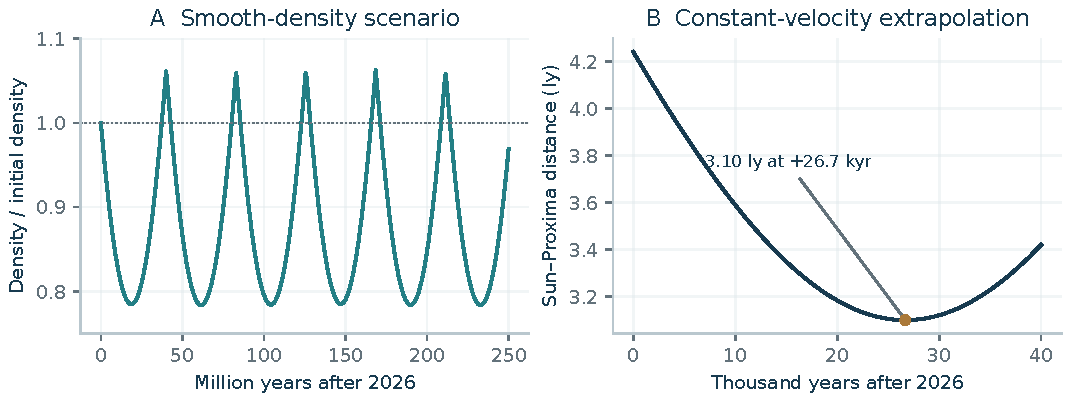
\includegraphics[width=\linewidth,height=68mm,keepaspectratio]{neighbourhood.pdf}\end{center}
\figcap{Two independent models with different clocks. A: adopted smooth-density profile along the Solar orbit. B: constant-velocity Sun--Proxima extrapolation. The apparent minimum in B is not a precision encounter forecast.}

\begin{minipage}[t]{.485\linewidth}\vspace{0pt}\setlength{\parskip}{3pt}
\subsection*{Density is not a discovery count}
A historical census of \ReportDensityLocalStars{} stars within 10 pc [5] sets the local reference:
\[
 n_0=\frac{\ReportDensityLocalStars{}}{(4\pi/3)(10\unit{pc})^3}
     =\ReportDensityLocal\unit{pc^{-3}}.
\]
The adopted thin/thick-disk scenario [6] ranges over \textbf{\ReportDensityMinRatio{}--\ReportDensityMaxRatio{}} times its initial density in 250 Myr: about \textbf{\ReportDensityMinStars{}--\ReportDensityMaxStars{} stars} in an instantaneous 10 pc sphere. It omits spiral-arm enhancements, clusters and migration. These are neither distinct arrivals nor planets found.
\end{minipage}\hfill
\begin{minipage}[t]{.485\linewidth}\vspace{0pt}\setlength{\parskip}{3pt}
\subsection*{Proxima is approaching now}
The adopted historical inputs [7] give about \textbf{\ReportProximaInitial{} ly} in 2026 and a radial velocity of \textbf{$\ReportProximaRadial\unit{km\,s^{-1}}$}; distance is decreasing. The total relative speed is about $\ReportProximaSpeed\unit{km\,s^{-1}}$.

Straight-line propagation gives a minimum near \textbf{\ReportProximaClosest{} ly after \ReportProximaClosestYears{} years}. This omits the Alpha Centauri system's orbital dynamics and Galactic differential acceleration. A negative radial speed today does not imply permanent approach.
\end{minipage}

\subsection*{The next 100, 1,000 and 10,000 years}
\begin{tabularx}{\linewidth}{@{}rXXX@{}}\toprule
Years & Solar path at \ReportSolarSpeed{} km/s & Median sightline shift & Accessibility change\\\midrule
100 & \ReportCenturyTablePath{} ly & \ReportCenturyTableSightline{} arcsec & $\ReportCenturyTableChange\%$\\
1,000 & \ReportMillenniumTablePath{} ly & \ReportMillenniumTableSightline{} arcsec & $\ReportMillenniumTableChange\%$\\
10,000 & \ReportTenMillenniaTablePath{} ly & $\ReportTenMillenniaTableSightline^\circ$ & $\ReportTenMillenniaTableChange\%$\\\bottomrule
\end{tabularx}\par\vspace{7pt}
The last two columns use the same selected \ReportSampleSize{} Gaia sources and baseline imaging thresholds as page 3. They are nominal constant-relative-velocity calculations, with \textbf{no new uncertainty propagation} for the longer intervals. Binary dynamics and differential Galactic acceleration are omitted. The score responds to distance and thresholds, not sky angle alone.

\takeaway{Still local}{In 10,000 years, the model Sun sweeps only $\ReportTenThousandAngle^\circ$ around the Galactic centre. A path of \ReportTenThousandPath{} light-years does not place it in a different spiral arm. Closer targets may be easier to study, but none of these results establishes life or predicts a habitable-planet discovery.}

\reportpage{05 / PHYSICS BEHIND THE PICTURES}{Reading the 3D simulation correctly}
A trajectory's appearance depends on the reference frame. The same planet follows a closed orbit in a co-moving view and a winding path when Solar travel is included. This does not imply a universal helix through spacetime.
\begin{center}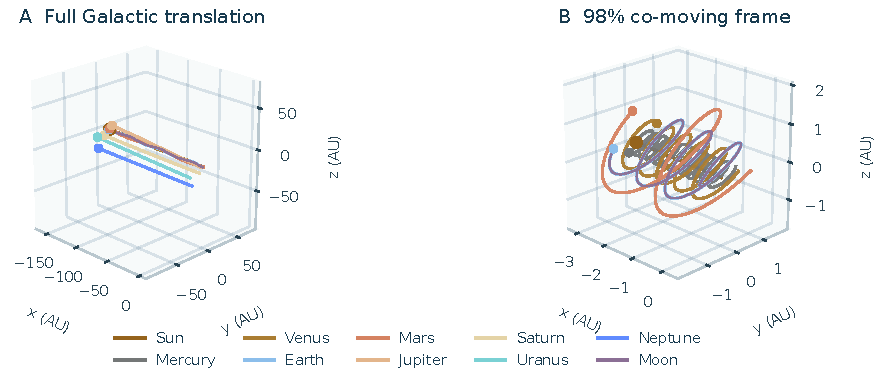
\includegraphics[width=\linewidth,height=67mm,keepaspectratio]{paths.pdf}\end{center}
\figcap{Three model years: A shows all ten bodies; B shows the Sun, inner planets and Moon. Each panel has equal AU axes with different displayed ranges. Markers are enlarged. Vector model plots, not website screenshots.}

\subsection*{Three motions that should not be confused}
\textbf{Planetary reflex:} the Sun moves around the Solar System barycentre in response to the planets. \textbf{Vertical Solar oscillation:} the long-clock orbit moves above and below the model Galactic midplane. \textbf{Galactic warp:} the displayed outer-disk bend is a separate kinematic illustration [8]. It does not supply an additional force to the Solar integration.

The long clock uses a nearly circular orbit in a static smooth potential. \textbf{A self-consistent evolution of the Galactic plane is not modelled.} The ecliptic's roughly $60^\circ$ tilt is relative to the Galactic plane; it is not the inclination of the Sun's entire Galactic orbit.

\begin{minipage}[t]{.485\linewidth}\vspace{0pt}\setlength{\parskip}{3pt}
\subsection*{A released probe keeps moving}
A passive probe inherits its release velocity and accelerates under gravity. Leaving it outside Earth does not leave it at a fixed Galactic coordinate.

The cyan 2026 marker is a \emph{hypothetical held reference}. Cancelling its velocity and holding it fixed would require a specified propulsion and force-compensation scheme. The simulation does not design such a mission.
\subsection*{The heliosphere is not a wall}
The model marks a 120 AU heliopause, a 90 AU termination shock and radial 400 km/s wind tracers inside the shock. Real boundaries are asymmetric and time dependent [9]; energetic cosmic rays can penetrate. No MHD or radiation-transport calculation is claimed.
\end{minipage}\hfill
\begin{minipage}[t]{.485\linewidth}\vspace{0pt}\setlength{\parskip}{3pt}
\subsection*{Gravity and clocks}
For an isolated, nonrotating spherical body, a held clock and an ideal circular-orbit clock satisfy
\begin{align}
 \left(\frac{d\tau}{dt}\right)_{\!\mathrm{held}}&=\sqrt{1-\frac{2GM}{rc^2}},\\
 \left(\frac{d\tau}{dt}\right)_{\!\mathrm{circular}}&=\sqrt{1-\frac{3GM}{rc^2}}.
\end{align}
Here $t$ refers to a clock at infinity. Relative to a stationary spherical-Earth surface clock, a circular clock loses \textbf{24.74 $\mu$s/day at 400 km} and gains \textbf{38.51 $\mu$s/day at 20,200 km} [10]. Rotation and operational corrections are excluded.

The whole-system view sums ten masses at a fixed test point using a weak-field clock rate. The potential sheet has arbitrary display depth.
\end{minipage}

\takeaway{A tested approximation, not full GR}{The separate coupled 1PN lab starts from JPL states [11]. Its two-body Mercury benchmark gives 42.9798 arcsec/century against 42.9807 analytically. The ten-year lunar discrepancy reaches 215 km. This is not a navigation ephemeris.}

\reportpage{06 / EXPLORE, REPRODUCE AND CRITIQUE}{A guide for readers and prospective mentors}
\begin{minipage}[t]{.485\linewidth}\vspace{0pt}\setlength{\parskip}{3pt}
\subsection*{Five ways to explore}
\begin{enumerate}[leftmargin=1.4em,itemsep=5pt]
\item \textbf{Inspect Galactic evidence.} Separate the 199 VLBI entries [12] from the ESA/Gaia reconstruction. \emph{Show warped disk} selects labelled $5\times$ height; restore $1\times$ for true proportions.
\item \textbf{Resolve 100 light-years.} Open the journey preview: this takes about 128,608 model years. The recording control captures the local scene while the tab remains visible.
\item \textbf{Change the frame.} In \emph{Sun \& all planets}, compare full Galactic and 98\% co-moving paths. \emph{Inspect a planet} follows a selected body at physical radius; \emph{Whole system} restores context.
\item \textbf{Read physical quantities.} \emph{Space \& Time} shows the whole system on a years clock; selecting Earth opens a local clock experiment. The 1PN lab integrates coupled dynamics separately.
\item \textbf{Test gas separately.} The gas lab solves 2D isothermal Euler flow on a $64\times64$ grid. Height graphs density, not warp. It is not a fitted 3D/MHD Galaxy simulation.
\end{enumerate}
\end{minipage}\hfill
\begin{minipage}[t]{.485\linewidth}\vspace{0pt}\setlength{\parskip}{3pt}
\subsection*{Questions for the community}
\textbf{A feasible next test.} Which known systems have planetary orbital planes and relative velocities well enough constrained to test entry into a transit band?

\textbf{A realistic observing programme.} Which apparent gains survive exposure-time budgets, repeated visits, binaries and instrument noise?

\textbf{A second observer.} What physically feasible probe orbit would add a useful baseline beyond Earth's orbit and long-term astrometry?

\textbf{Relevant prior work.} Which studies best connect changing sightlines, nearby encounters and exoplanet detection opportunities?

\textit{I am an independent researcher without a formal supervisor. I built this software out of curiosity and would welcome expert guidance on what is useful, what is already established, and what needs correction.}
\end{minipage}
\vspace{7pt}
\subsection*{Selected sources and provenance}
\begingroup\sffamily\fontsize{8}{9.6}\selectfont
\begin{multicols}{2}
\reference{1}{ESA/Gaia/DPAC; S. Payne-Wardenaar (2025). Milky Way reconstruction. CC BY-SA 3.0 IGO; annotated here.}{https://www.esa.int/ESA_Multimedia/Images/2025/01/The_best_Milky_Way_map_by_Gaia}
\reference{2}{Finding Earth 2.0. Saved analysis, 28 Aug 2026. Original habitable-zone plot; repository and methods.}{https://github.com/Biswajit1999/finding-earth-2/tree/14828643bdd9342eeb2aff65c5dd32eef31dd2c3}
\reference{3}{Kaltenegger \& Faherty (2021). Past, present and future stars that can see Earth as a transiting exoplanet.}{https://doi.org/10.1038/s41586-021-03596-y}
\reference{4}{Gaia DR3 (2022). Catalogue release; sample selection and covariance treatment in the full methods.}{https://doi.org/10.5270/esa-qa4lep3}
\reference{5}{Reyl\'e et al. (2021). The 10 parsec sample in the Gaia era. Historical local-census normalization.}{https://doi.org/10.1051/0004-6361/202140985}
\reference{6}{Juri\'c et al. (2008). Milky Way tomography with SDSS. Basis of the adopted smooth-density scenario.}{https://arxiv.org/abs/astro-ph/0510520}
\reference{7}{Kervella, Th\'evenin \& Lovis (2017). Proxima / Alpha Centauri measurement inputs.}{https://doi.org/10.1051/0004-6361/201629930}
\reference{8}{Poggio et al. (2025). The great wave: outer-disk warp and corrugation. Not fitted by this simulation.}{https://doi.org/10.1051/0004-6361/202451668}
\reference{9}{NASA. Uncovering our Solar System's shape. Heliosphere structure and observational context.}{https://www.nasa.gov/solar-system/uncovering-our-solar-systems-shape/}
\reference{10}{Ashby (2003). Relativity in the Global Positioning System.}{https://doi.org/10.12942/lrr-2003-1}
\reference{11}{Park et al. (2021). JPL DE440/DE441 planetary and lunar ephemerides.}{https://doi.org/10.3847/1538-3881/abd414}
\reference{12}{Reid et al. (2019). Trigonometric parallaxes and Galactic spiral structure. VLBI data and arm fits.}{https://arxiv.org/abs/1910.03357}
\end{multicols}
\endgroup
\vspace{2pt}
\source{Figure 2 is the original saved plot; figures 3--5 are vector plots of project calculations. The original discussion note is preserved unchanged. Planet maps in the simulation: Solar System Scope / INOVE, CC BY 4.0, with illustrative surface and orientation choices. No institutional endorsement is implied.}

\takeaway{Open the project}{\href{https://biswajit1999.github.io/moving-observer/}{Simulation and full methods}\quad\textbar\quad\href{https://github.com/Biswajit1999/moving-observer}{Source, data and LaTeX}\quad\textbar\quad\href{https://github.com/Biswajit1999/moving-observer/issues/new/choose}{Questions and scientific criticism}}

\end{document}
